\section{Experiments} \label{sec:experiments}
\subsection*{Training}
Entrambe le reti sono state addestrate per 30 epoche utilizzando la cross-entropy loss. CustomNet è stata addestrata da zero e la Figura \ref{fig7:layer1_filter} mostra i filtri del primo layer convoluzionale al termine dell'addestramento. 
\begin{figure}[!hbt]
    \centering
    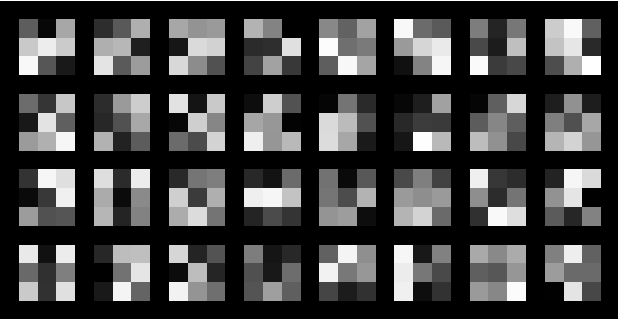
\includegraphics[width=\columnwidth]{images/layer1_filter.png}
    \caption{Filtri del primo layer convoluzionale di CustomNet ottenuti al termine della fase di training}
    \label{fig7:layer1_filter}
\end{figure}\par
La figura \ref{fig8:feature_map} mostra la decima feature map per ogni layer convoluzionale; la prima immagine mostra l'input, in questo caso corrispondente alla classe Coat (4). Si osserva come man mano che si scende in profondità la rete impara ad estrarre l'oggetto presente e distinguerlo dal background.
\begin{figure}[!hbt]
    \centering
    \includegraphics[width=\columnwidth]{images/customNet_featureMap2.png}
    \caption{Input e feature map dei layer convoluzionali}
    \label{fig8:feature_map}
\end{figure}\par
Per quanto riguarda Resnet sono stati addestrati solo i layer alterati rispetto alla struttura originale, essendo la rete preaddestrata con il dataset ImageNet \cite{deng2009imagenet}. Grazie a questa procedura di transfer learning è stato possibile utilizzare la rete che altrimenti avrebbe richiesto un tempo eccessivo per la fase di training.
\subsection*{Risultati}
Per valutare le performance delle reti è stata utilizzata l'accuracy, questa consente di individuare la percentuale di classificazioni corrette sul totale delle predizioni. \`{E} definita come:$$Accuracy = \frac{predizioni\: corrette}{predizioni\: totali}$$ Le Figure \ref{fig9:customNet_score} e \ref{fig10:resNet_score} mostrano l'andamento dell'accuracy su train e test set per entrambi i modelli all'avanzare delle epoche. CustomNet riesce a raggiungere un'accuracy del 91\% sul train set e dell'88\% sul test. Resnet-18 ottiene dei risultati inferiori arrivando ad un 74\% sul training e un 68\% sul test.
\begin{figure}[!hbt]
    \centering
    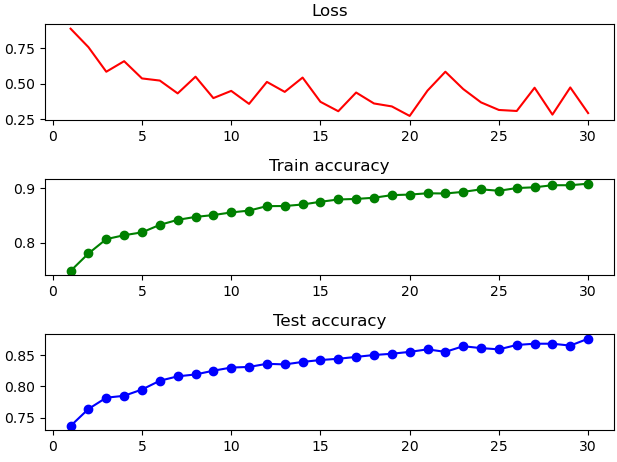
\includegraphics[width=\columnwidth]{images/CustomNetScore1bis.png}
    \caption{Andamento di loss, train accuracy e test accuracy utilizzando CustomNet}
    \label{fig9:customNet_score}
\end{figure}
\begin{figure}[!hbt]
    \centering
    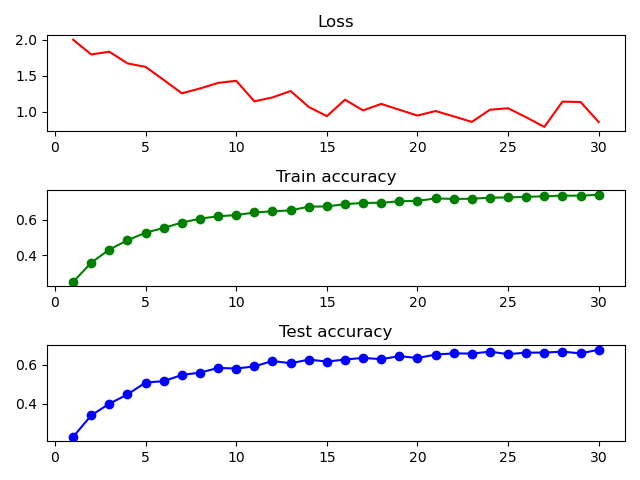
\includegraphics[width=\columnwidth]{images/ResNetScore.png}
    \caption{Andamento di loss, train accuracy e test accuracy utilizzando ResNet-18}
    \label{fig10:resNet_score}
\end{figure}\par
Sono state inoltre calcolate precision e recall per le singole classi:
$$Precision = \frac{TP}{TP+FP} \quad Recall=\frac{TP}{TP+FN}$$
La precision indica la proporzione di predizioni positive corrette rispetto a tutte le predizioni positive. La recall indica invece la proporzione di predizioni positive corrette rispetto a tutti i campioni effettivamente positivi. In un task di classificazione multiclasse si assegna la classe positiva ad una sola etichetta e al resto delle label viene assegnata la classe negativa.
\begin{table}[!hbt]
\centering
\begin{adjustbox}{width=\columnwidth}
\begin{tabular}{|l|c|c|c|c|}
\hline        & \multicolumn{2}{c|}{\textbf{CustomNet}}& \multicolumn{2}{c|}{\textbf{ResNet-18}}\\
\hline \textbf{Label} &\textbf{Precision} &\textbf{Recall} &\textbf{Precision} &\textbf{Recall} \\
\hline 0: T-shirt/Top & 0.85& 0.90 & 0.67&0.73\\
\hline 1: Trouser     & 0.98& 0.99 & 0.90&0.81\\
\hline 2: Pullover    & 0.82& 0.81 & 0.54&0.43\\
\hline 3: Dress       & 0.84& 0.85 & 0.67&0.64\\
\hline 4: Coat        & 0.83& 0.86 & 0.52&0.65\\
\hline 5: Sandal      & 0.89& 0.94 & 0.76&0.80\\
\hline 6: Shirt       & 0.76& 0.68 & 0.34&0.37\\
\hline 7: Sneaker     & 0.92& 0.90 & 0.85&0.84\\
\hline 8: Bag         & 0.95& 0.96 & 0.75&0.79\\
\hline 9: Ankle boot  & 0.95& 0.92 & 0.82&0.82\\
\hline
\end{tabular}
\end{adjustbox}
\label{tab1:precision-recall}
\caption{Precision e recall calcolate sul test set}
\end{table}\par
Infine è stata visualizzata la confusion matrix per CustomNet riguardante le predizioni effettuate sul test set. Grazie a questa si riesce a capire quali classi siano più difficili da disambiguare per la rete. La diagonale principale rappresenta il numero di predizioni corrette per ogni classe, mentre invece i valori fuori diagonale rappresentano una predizione sbagliata.
\begin{figure}[!hbt]
    \centering
    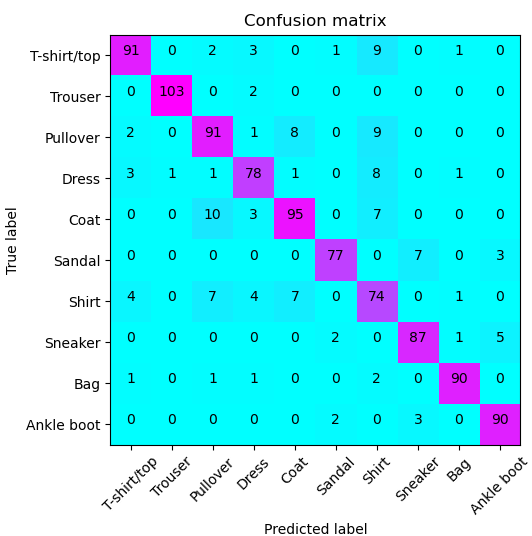
\includegraphics[width=\columnwidth]{images/confusion_matrix1.png}
    \caption{Confusion matrix per le predizioni di CustomNet sul test set}
    \label{fig11:confusion_matrix}
\end{figure}

